% https://wiki.physik.uzh.ch/cms/latex:tikz:electromagnetic_wave
    % Author: Izaak Neutelings (May 2018)
% Inspiration: https://tex.stackexchange.com/questions/113900/draw-polarized-light
\documentclass[border=3pt,tikz]{article}
\usepackage[top=0.25in, bottom=0.25in]{geometry}
\usepackage{amsmath} % for \text
\usepackage{tikz}

\tikzset{>=latex} % for LaTeX arrow head

\usepackage{xcolor}

\colorlet{myblue}{black!40!blue}
\colorlet{myred}{black!40!red}

\begin{document}
	
	
	% Electromagnetic wave - black
	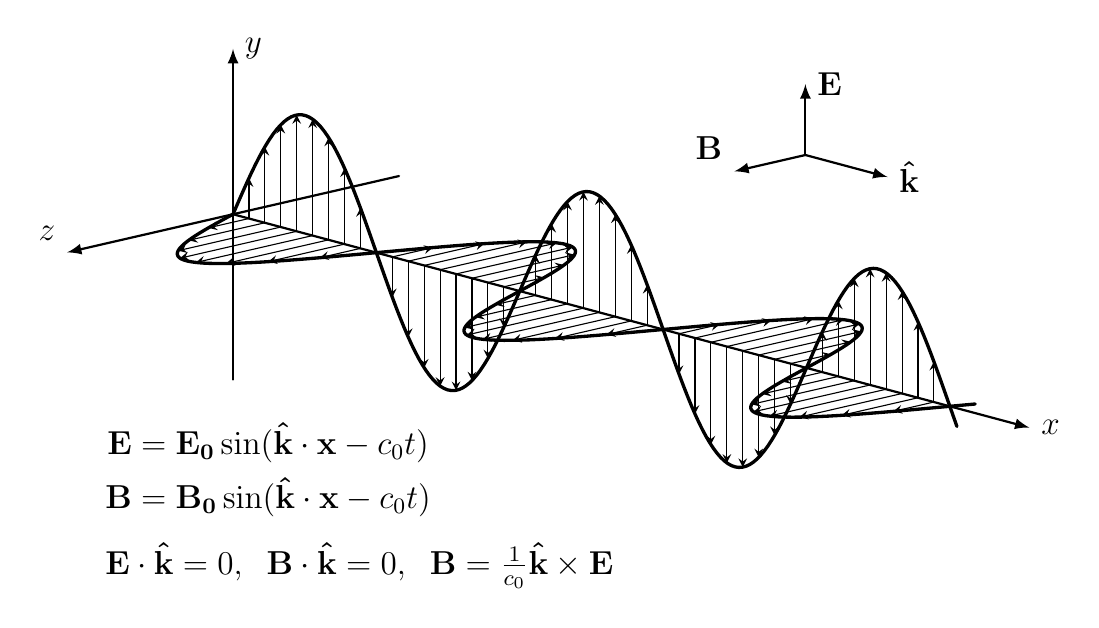
\begin{tikzpicture}[x=(-15:1.2), y=(90:1.0), z=(-150:1.0),
	line cap=round, line join=round,
	axis/.style={black, thick,->},
	vector/.style={>=stealth,->}]
	\large
	\def\A{1.5}
	\def\nNodes{5} % use even number
	\def\nVectorsPerNode{8}
	\def\N{\nNodes*40}
	\def\xmax{\nNodes*pi/2*1.01}
	\pgfmathsetmacro\nVectors{(\nVectorsPerNode+1)*\nNodes}
	
	\def\vE{\mathbf{E}}
	\def\vB{\mathbf{B}}
	\def\vk{\mathbf{\hat{k}}}
	
	% main axes
	\draw[axis] (0,0,0) -- ++(\xmax*1.1,0,0) node[right] {$x$};
	\draw[axis] (0,-\A*1.4,0) -- (0,\A*1.4,0) node[right] {$y$};
	\draw[axis] (0,0,-\A*1.4) -- (0,0,\A*1.4) node[above left] {$z$};
	
	% small axes
	\def\xOffset{{(\nNodes-2)*pi/2}}
	\def\yOffset{\A*1.2}
	\def\zOffset{\A*1.2}
	\draw[axis] (\xOffset,\yOffset,-\zOffset) -- ++(\A*0.6,0,0) node[right] {$\vk$};
	\draw[axis] (\xOffset,\yOffset,-\zOffset) -- ++(0,\A*0.6,0) node[right] {$\vE$};
	\draw[axis] (\xOffset,\yOffset,-\zOffset) -- ++(0,0,\A*0.6) node[above left] {$\vB$};
	
	% equation
	\node[above right] at (\xOffset,-0.5*\yOffset,4*\zOffset)
	{$\begin{aligned}
		\vE &= \mathbf{E_0}\sin(\vk\cdot\mathbf{x}-c_0t)\\
		\vB &= \mathbf{B_0}\sin(\vk\cdot\mathbf{x}-c_0t)\\
		\end{aligned}$};
	\node[below right] at (\xOffset,-0.5*\yOffset,4*\zOffset)
	{$\vE\cdot\vk = 0,\;\; \vB\cdot\vk = 0,\;\; \vB = \frac{1}{c_0}\vk\times\vE$};
	
	% waves
	\draw[very thick,variable=\t,domain=0:\nNodes*pi/2*1.01,samples=\N]
	plot (\t,{\A*sin(\t*360/pi)},0);
	\draw[very thick,variable=\t,domain=0:\nNodes*pi/2*1.01,samples=\N]
	plot (\t,0,{\A*sin(\t*360/pi)});
	
	% draw vectors
	\foreach \k [evaluate={\t=\k*pi/2/(\nVectorsPerNode+1);
		\angle=\k*90/(\nVectorsPerNode+1);
		\c=(mod(\angle,90)!=0);}]
	in {1,...,\nVectors}{
		\if\c1
		\draw[vector] (\t,0,0) -- ++(0,{\A*sin(2*\angle)},0);
		\draw[vector] (\t,0,0) -- ++(0,0,{\A*sin(2*\angle)});
		\fi
	}
	
	\end{tikzpicture}
	
	
	
	% Electromagnetic wave - circular polarization
	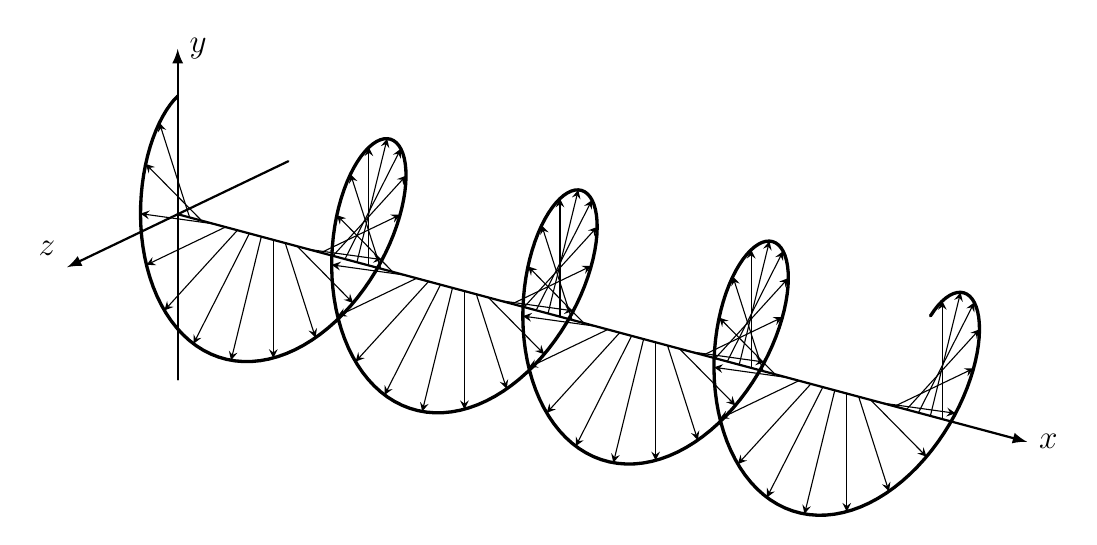
\begin{tikzpicture}[x=(-15:0.8), y=(90:1.0), z=(-150:1.0),
	line cap=round, line join=round,
	axis/.style={black, thick,->},
	vector/.style={>=stealth,->}]
	\large
	\def\A{1.5}
	\def\nNodes{8} % use even number
	\def\nVectorsPerNode{8}
	\def\N{\nNodes*40}
	\def\xmax{\nNodes*pi/2*1.01}
	\pgfmathsetmacro\nVectors{\nVectorsPerNode*\nNodes}
	
	\def\vE{\mathbf{E}}
	\def\vB{\mathbf{B}}
	\def\vk{\mathbf{\hat{k}}}
	
	% main axes
	\draw[axis] (0,0,0) -- ++(\xmax*1.1,0,0) node[right] {$x$};
	\draw[axis] (0,-\A*1.4,0) -- (0,\A*1.4,0) node[right] {$y$};
	\draw[axis] (0,0,-\A*1.4) -- (0,0,\A*1.4) node[above left] {$z$};
	
	% waves
	\draw[very thick,variable=\t,domain=0:\nNodes*pi/2*1.01,samples=\N]
	plot (\t,{\A*cos(\t*360/pi)},{\A*sin(\t*360/pi)});
	
	% draw vectors
	\foreach \k [evaluate={\t=\k*pi/2/\nVectorsPerNode;
		\angle=\k*90/\nVectorsPerNode;}]
	in {1,...,\nVectors}{
		\draw[vector] (\t,0,0) -- ++(0,{\A*cos(2*\angle)},{\A*sin(2*\angle)});
	}
	
	\end{tikzpicture}
	
	
	
	% Electromagnetic wave - colored
	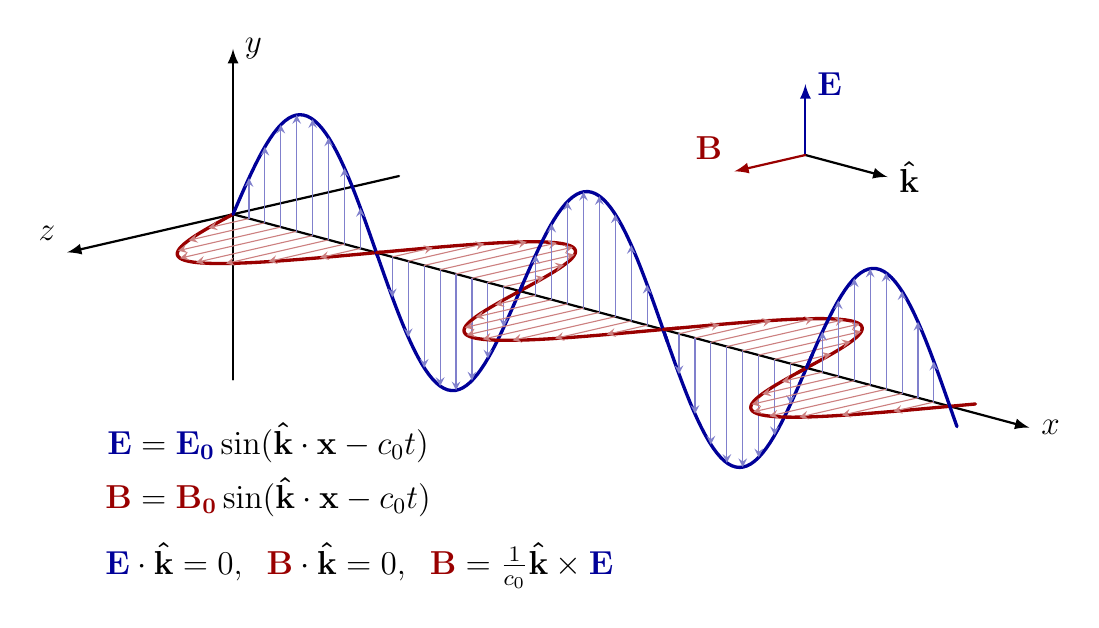
\begin{tikzpicture}[x=(-15:1.2), y=(90:1.0), z=(-150:1.0),
	line cap=round, line join=round,
	axis/.style={black, thick,->},
	vector/.style={>=stealth,->}]
	\large
	\def\A{1.5}
	\def\nNodes{5} % use even number
	\def\nVectorsPerNode{8}
	\def\N{\nNodes*40}
	\def\xmax{\nNodes*pi/2*1.01}
	\pgfmathsetmacro\nVectors{(\nVectorsPerNode+1)*\nNodes}
	
	\def\vE{{\color{myblue}\mathbf{E}}}
	\def\vB{{\color{myred}\mathbf{B}}}
	\def\vk{\mathbf{\hat{k}}}
	
	\def\drawENode{ % draw E node and vectors with some offset
		\draw[myblue,very thick,variable=\t,domain=\iOffset*pi/2:(\iOffset+1)*pi/2*1.01,samples=40]
		plot (\t,{\A*sin(\t*360/pi)},0);
		\foreach \k [evaluate={\t=\k*pi/2/(\nVectorsPerNode+1);
			\angle=\k*90/(\nVectorsPerNode+1);}]
		in {1,...,\nVectorsPerNode}{
			\draw[vector,myblue!50]  (\iOffset*pi/2+\t,0,0) -- ++(0,{\A*sin(2*\angle+\iOffset*180)},0);
		}
	}
	\def\drawBNode{ % draw B node and vectors with some offset
		\draw[myred,very thick,variable=\t,domain=\iOffset*pi/2:(\iOffset+1)*pi/2*1.01,samples=40]
		plot (\t,0,{\A*sin(\t*360/pi)});
		\foreach \k [evaluate={\t=\k*pi/2/(\nVectorsPerNode+1);
			\angle=\k*90/(\nVectorsPerNode+1);}]
		in {1,...,\nVectorsPerNode}{
			\draw[vector,myred!50]  (\iOffset*pi/2+\t,0,0) -- ++(0,0,{\A*sin(2*\angle+\iOffset*180)});
		}
	}
	
	% main axes
	\draw[axis] (0,0,0) -- ++(\xmax*1.1,0,0) node[right] {$x$};
	\draw[axis] (0,-\A*1.4,0) -- (0,\A*1.4,0) node[right] {$y$};
	\draw[axis] (0,0,-\A*1.4) -- (0,0,\A*1.4) node[above left] {$z$};
	
	% small axes
	\def\xOffset{{(\nNodes-2)*pi/2}}
	\def\yOffset{\A*1.2}
	\def\zOffset{\A*1.2}
	\draw[axis,black] (\xOffset,\yOffset,-\zOffset) -- ++(\A*0.6,0,0) node[right,align=center] {$\mathbf{\hat{k}}$}; %\\propagation
	\draw[axis,myblue]  (\xOffset,\yOffset,-\zOffset) -- ++(0,\A*0.6,0) node[right] {$\mathbf{E}$};
	\draw[axis,myred]   (\xOffset,\yOffset,-\zOffset) -- ++(0,0,\A*0.6) node[above left] {$\mathbf{B}$};
	
	% equation
	\node[above right] at (\xOffset,-0.5*\yOffset,4*\zOffset)
	{$\begin{aligned}
		\vE &= {\color{myblue}\mathbf{E_0}}\sin(\vk\cdot\mathbf{x}-c_0t)\\
		\vB &= {\color{myred} \mathbf{B_0}}\sin(\vk\cdot\mathbf{x}-c_0t)\\
		\end{aligned}$};
	\node[below right] at (\xOffset,-0.5*\yOffset,4*\zOffset)
	{$\vE\cdot\vk = 0,\;\; \vB\cdot\vk = 0,\;\; \vB = \frac{1}{c_0}\vk\times\vE$};
	
	% draw (anti-)nodes
	\foreach \iNode [evaluate={\iOffset=\iNode-1;}] in {1,...,\nNodes}{
		\ifodd\iNode \drawBNode \drawENode % E overlaps B
		\else        \drawENode \drawBNode % B overlaps E
		\fi
	}
	
	\end{tikzpicture}
	
	
	
\end{document}

